\section*{Appendice}
\addcontentsline{toc}{section}{Appendice}

\begin{figure}[H]
    \centering
    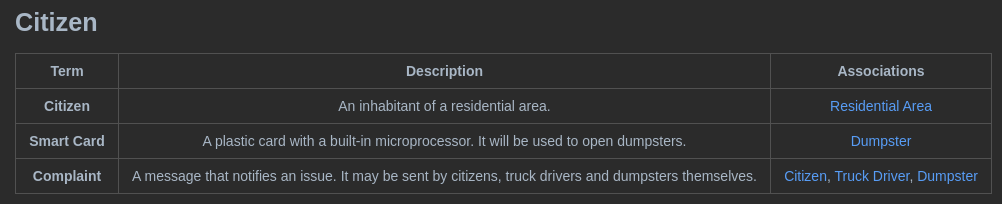
\includegraphics[width=\textwidth]{../img/citizen-ubiquitous-language.pm}
    \caption{\textit{Ubiquitous Language}: i termini del topic "cittadino". \hyperlink{back:citizen-ubiquitous-language}{Torna indietro}.}
    \label{fig:citizen-ubiquitous-language}
\end{figure}

\begin{figure}[H]
    \centering
    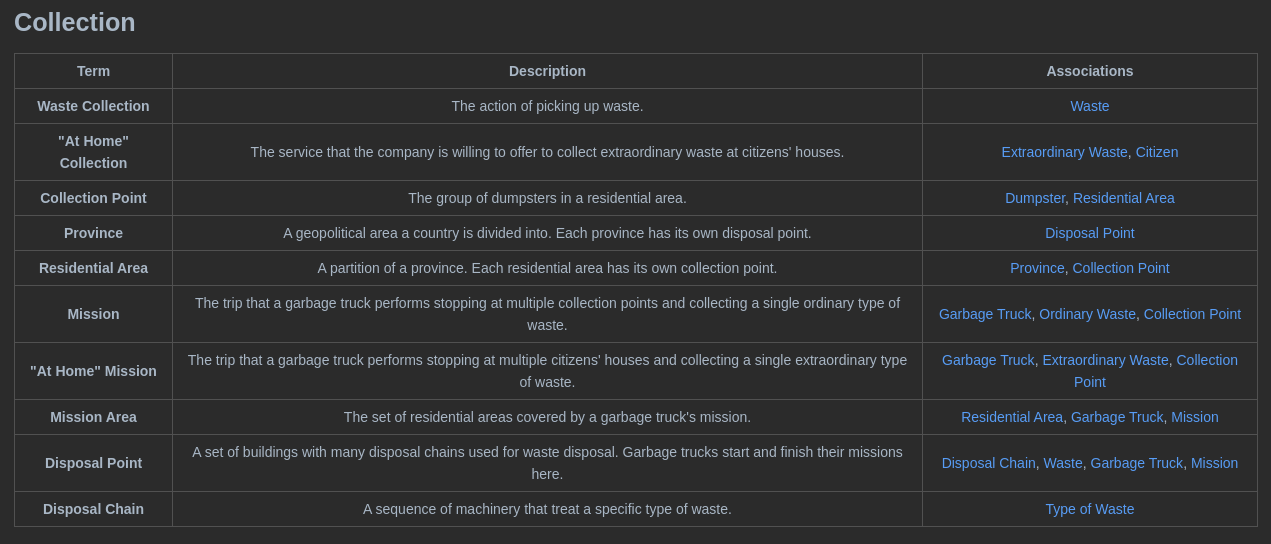
\includegraphics[width=\textwidth]{../img/collection-ubiquitous-language.pm}
    \caption{\textit{Ubiquitous Language}: i termini del topic "raccolta". \hyperlink{back:collection-ubiquitous-language}{Torna indietro}.}
    \label{fig:collection-ubiquitous-language}
\end{figure}

\begin{figure}[H]
    \centering
    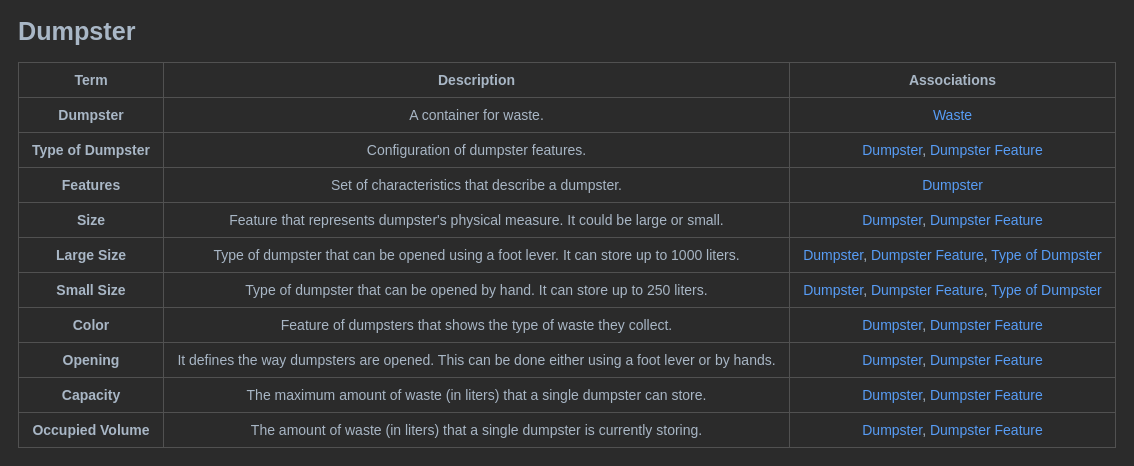
\includegraphics[width=\textwidth]{../img/dumpster-ubiquitous-language.pm}
    \caption{\textit{Ubiquitous Language}: i termini del topic "cassonetti". \hyperlink{back:dumpster-ubiquitous-language}{Torna indietro}.}
    \label{fig:dumpster-ubiquitous-language}
\end{figure}

\begin{figure}[H]
    \centering
    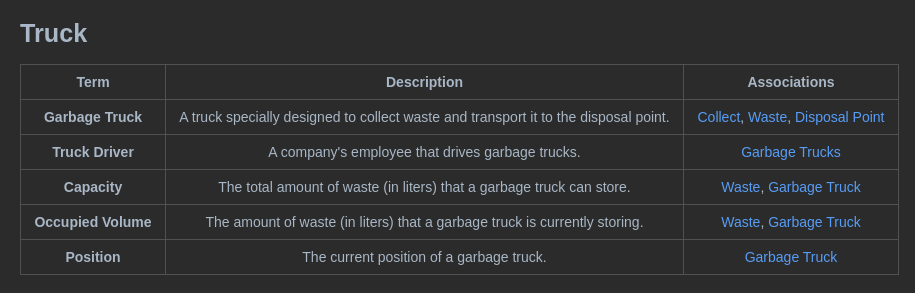
\includegraphics[width=\textwidth]{../img/truck-ubiquitous-language.pm}
    \caption{\textit{Ubiquitous Language}: i termini del topic "camioncini". \hyperlink{back:truck-ubiquitous-language}{Torna indietro}.}
    \label{fig:truck-ubiquitous-language}
\end{figure}

\begin{figure}[H]
    \centering
    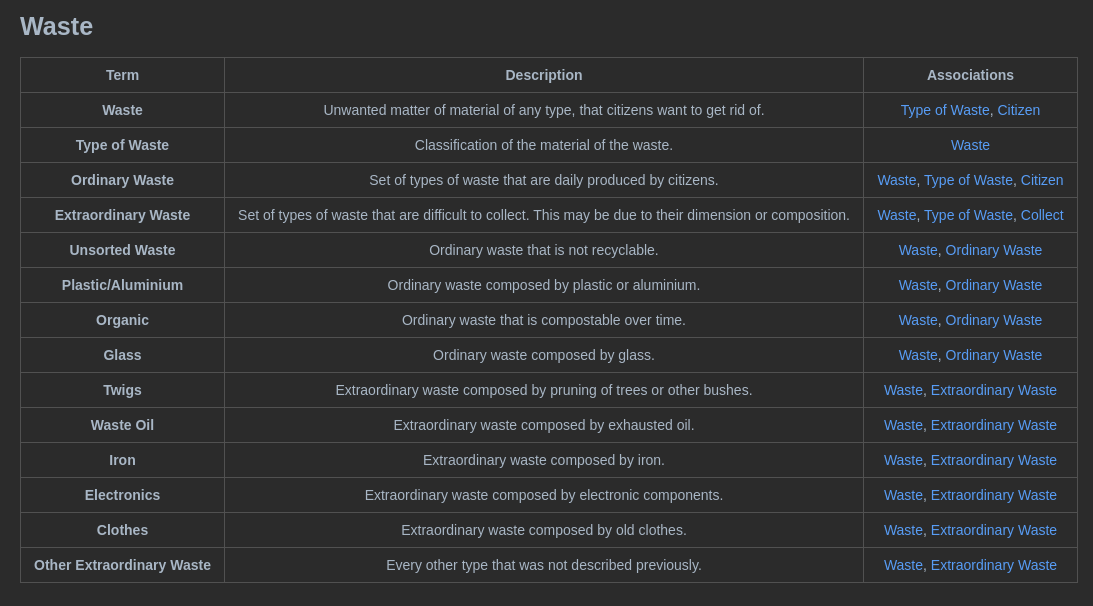
\includegraphics[width=\textwidth]{../img/waste-ubiquitous-language.pm}
    \caption{\textit{Ubiquitous Language}: i termini del topic "rifiuti". \hyperlink{back:waste-ubiquitous-language}{Torna indietro}.}
    \label{fig:waste-ubiquitous-language}
\end{figure}

\begin{figure}[H]
    \centering
    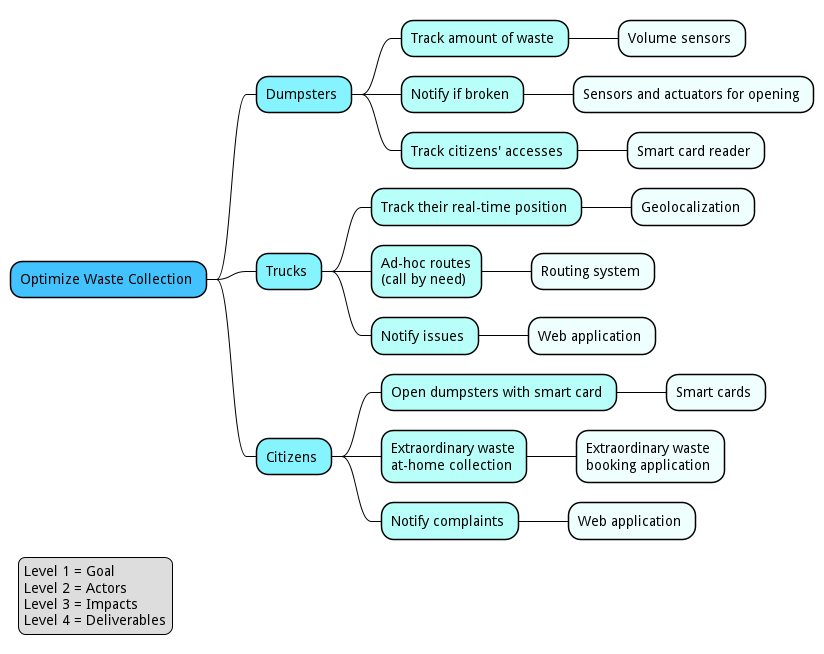
\includegraphics[width=\textwidth]{../img/impact-mapping.pm}
    \caption{\textit{Impact map} che, a partire dal \textit{goal}, mostra quali sono le soluzioni con maggiore impatto sugli attori del sistema. \hyperlink{back:impact-mapping}{Torna indietro}.}
    \label{fig:impact-mapping}
\end{figure}

\begin{figure}[H]
    \centering
    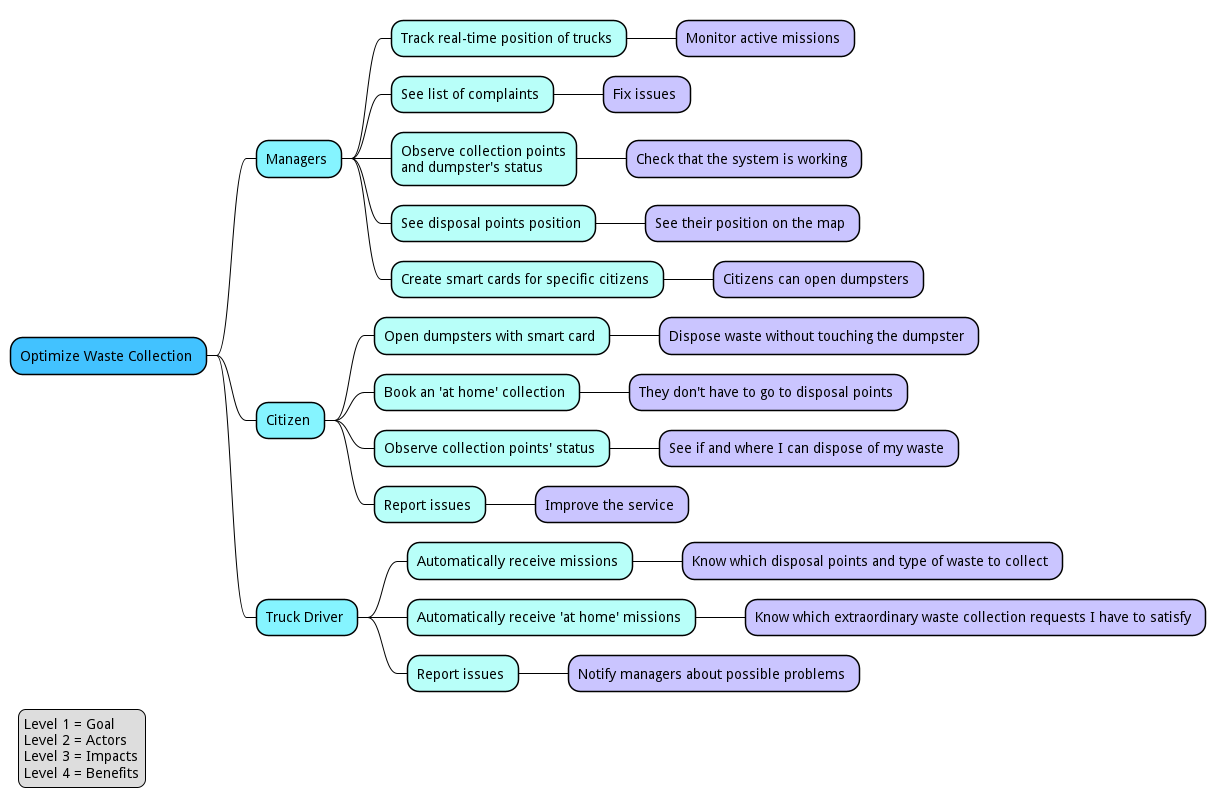
\includegraphics[width=\textwidth]{../img/benefit-mapping.pm}
    \caption{\textit{Impact map} che, a partire dal \textit{goal}, mostra chi sono gli attori che beneficiano maggiormente dai cambiamenti introdotti dal sistema. \hyperlink{back:benefit-mapping}{Torna indietro}.}
    \label{fig:benefit-mapping}
\end{figure}

\begin{figure}[H]
    \centering
    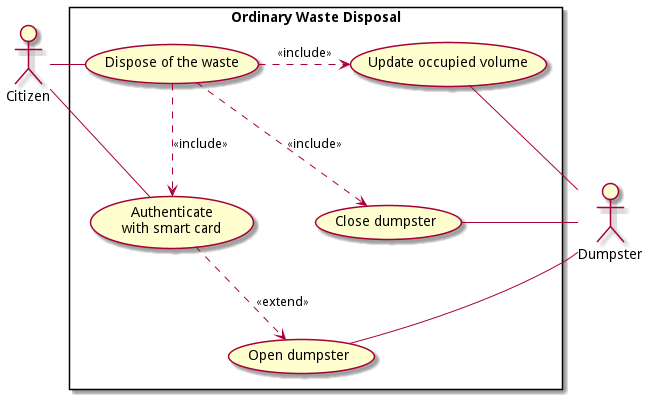
\includegraphics[width=\textwidth]{../img/ordinary-disposal-use-cases.pm}
    \caption{Diagramma dei casi d'uso dello scenario del conferimento di rifiuti ordinari. \hyperlink{back:ordinary-disposal-use-cases}{Torna indietro}.}
    \label{fig:ordinary-disposal-use-cases}
\end{figure}

\begin{figure}[H]
    \centering
    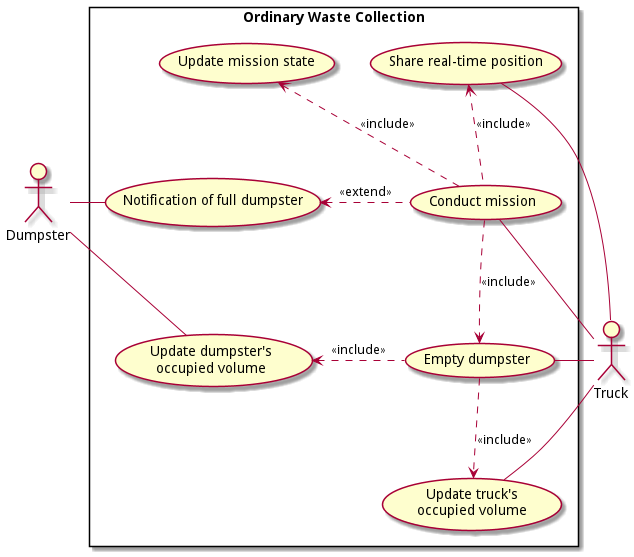
\includegraphics[width=\textwidth]{../img/ordinary-collection-use-cases.pm}
    \caption{Diagramma dei casi d'uso dello scenario della raccolta di rifiuti ordinari. \hyperlink{back:ordinary-collection-use-cases}{Torna indietro}.}
    \label{fig:ordinary-collection-use-cases}
\end{figure}

\begin{figure}[H]
    \centering
    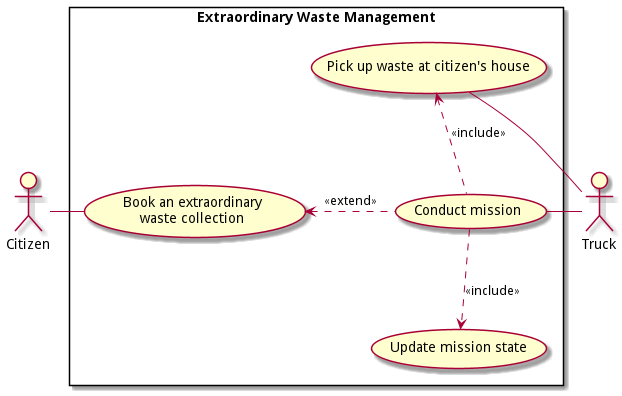
\includegraphics[width=\textwidth]{../img/extraordinary-management-use-cases.pm}
    \caption{Diagramma dei casi d'uso dello scenario della gestione di rifiuti straordinari. \hyperlink{back:extraordinary-management-use-cases}{Torna indietro}.}
    \label{fig:extraordinary-management-use-cases}
\end{figure}

\begin{figure}[H]
    \centering
    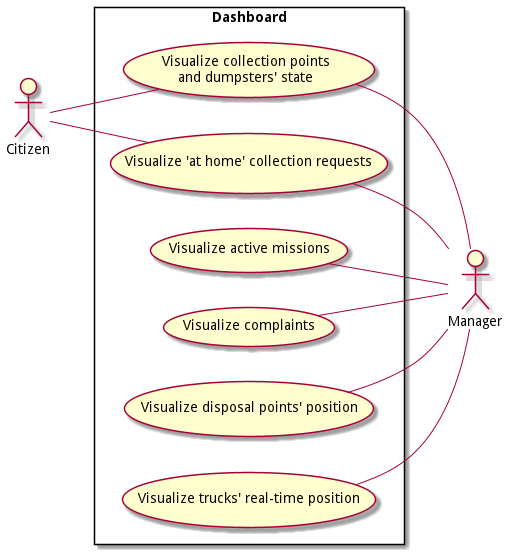
\includegraphics[width=\textwidth]{../img/dashboard-use-cases.pm}
    \caption{Diagramma dei casi d'uso dello scenario dell'utilizzo della dashboard. \hyperlink{back:dashboard-use-cases}{Torna indietro}.}
    \label{fig:dashboard-use-cases}
\end{figure}

\begin{figure}[H]
    \centering
    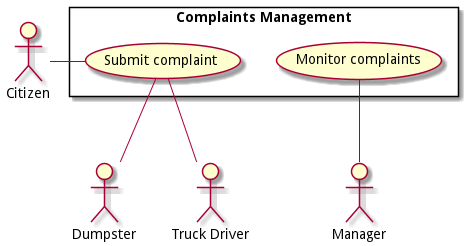
\includegraphics[width=\textwidth]{../img/complaints-use-cases.pm}
    \caption{Diagramma dei casi d'uso dello scenario della gestione dei reclami. \hyperlink{back:complaints-use-cases}{Torna indietro}.}
    \label{fig:complaints-use-cases}
\end{figure}

\begin{figure}[H]
    \centering
    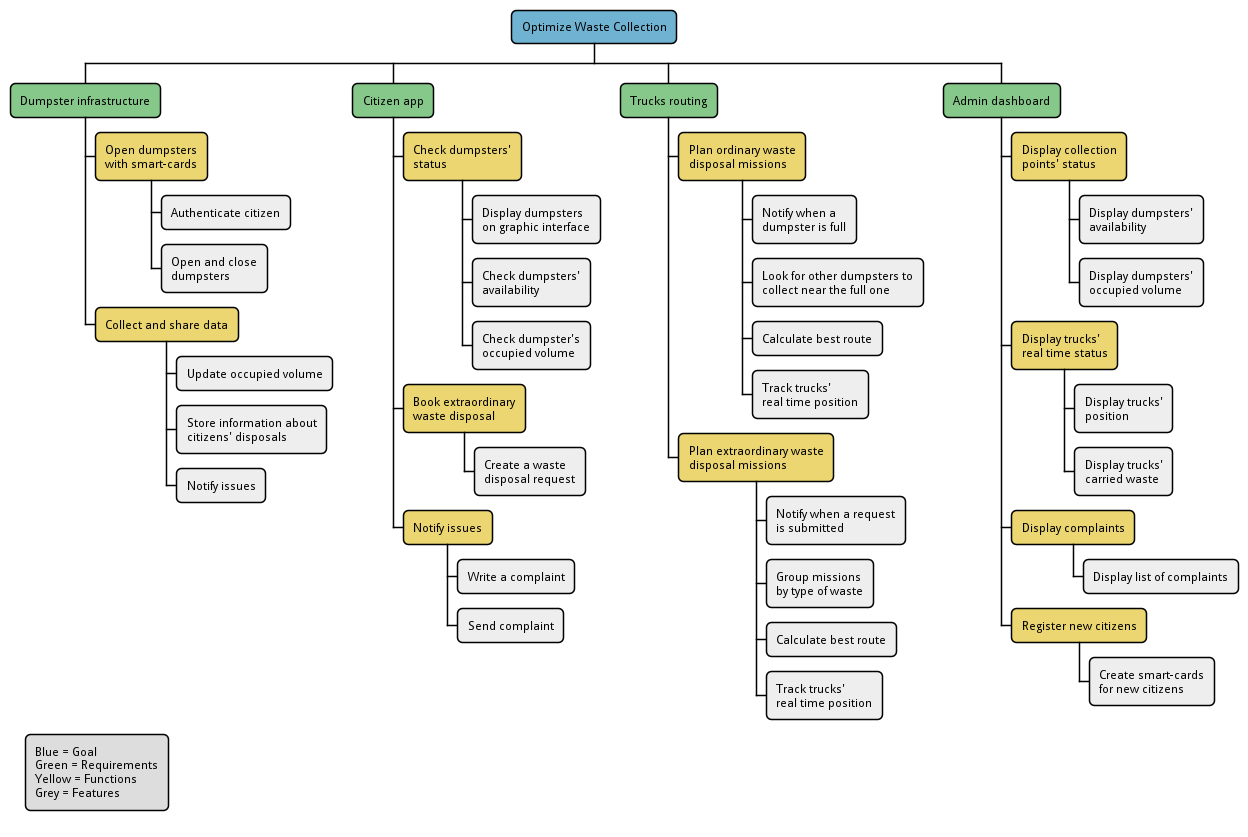
\includegraphics[width=\textwidth]{../img/requirement-breakdown-structure.pm}
    \caption{\textit{Requirement Breakdown Structure} derivata dall'analisi delle \textit{user stories} e parzialmente inclusa nel \textit{Project Overview Statement}   \hyperlink{back:requirement-breakdown-structure}{Torna indietro}.}
    \label{fig:requirement-breakdown-structure}
\end{figure}

\begin{figure}[H]
    \centering
    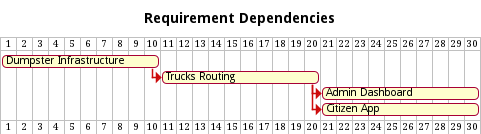
\includegraphics[width=\textwidth]{../img/gantt-requirements-dependencies.pm}
    \caption{Diagramma delle dipendenze tra i requisiti del progetto. \hyperlink{back:gantt-requirements-dependencies}{Torna indietro}.}
    \label{fig:gantt-requirements-dependencies}
\end{figure}

\begin{figure}[H]
    \centering
    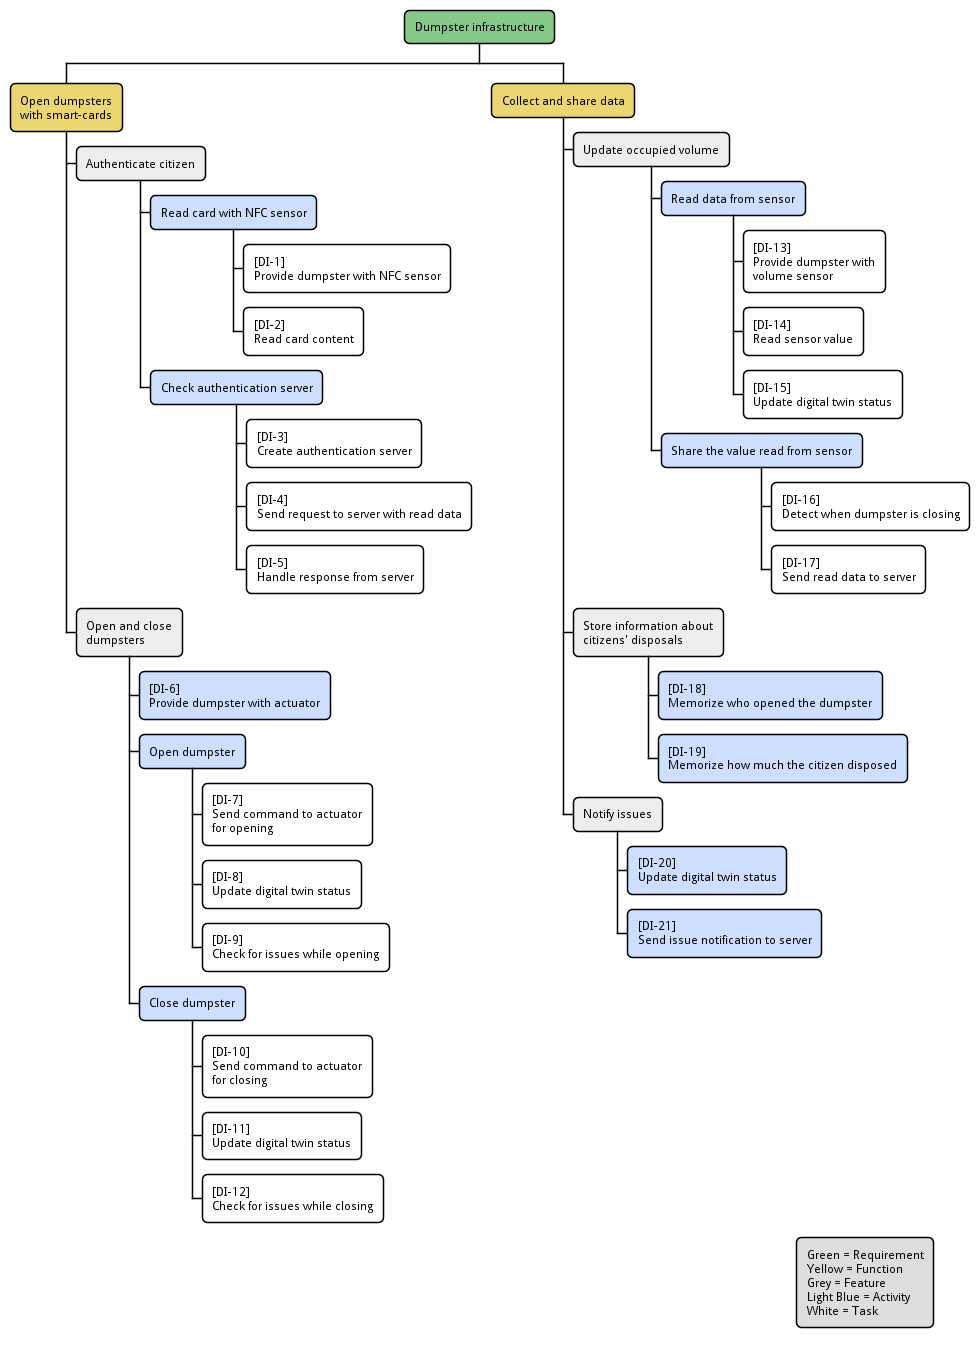
\includegraphics[width=\textwidth]{../img/wbs-dumpster-infrastructure.pm}
    \caption{\textit{Work Breakdown Structure} della \textbf{Dumpster Infrastructure}. \hyperlink{back:wbs-dumpster-infrastructure}{Torna indietro}.}
    \label{fig:wbs-dumpster-infrastructure}
\end{figure}

\begin{figure}[H]
    \centering
    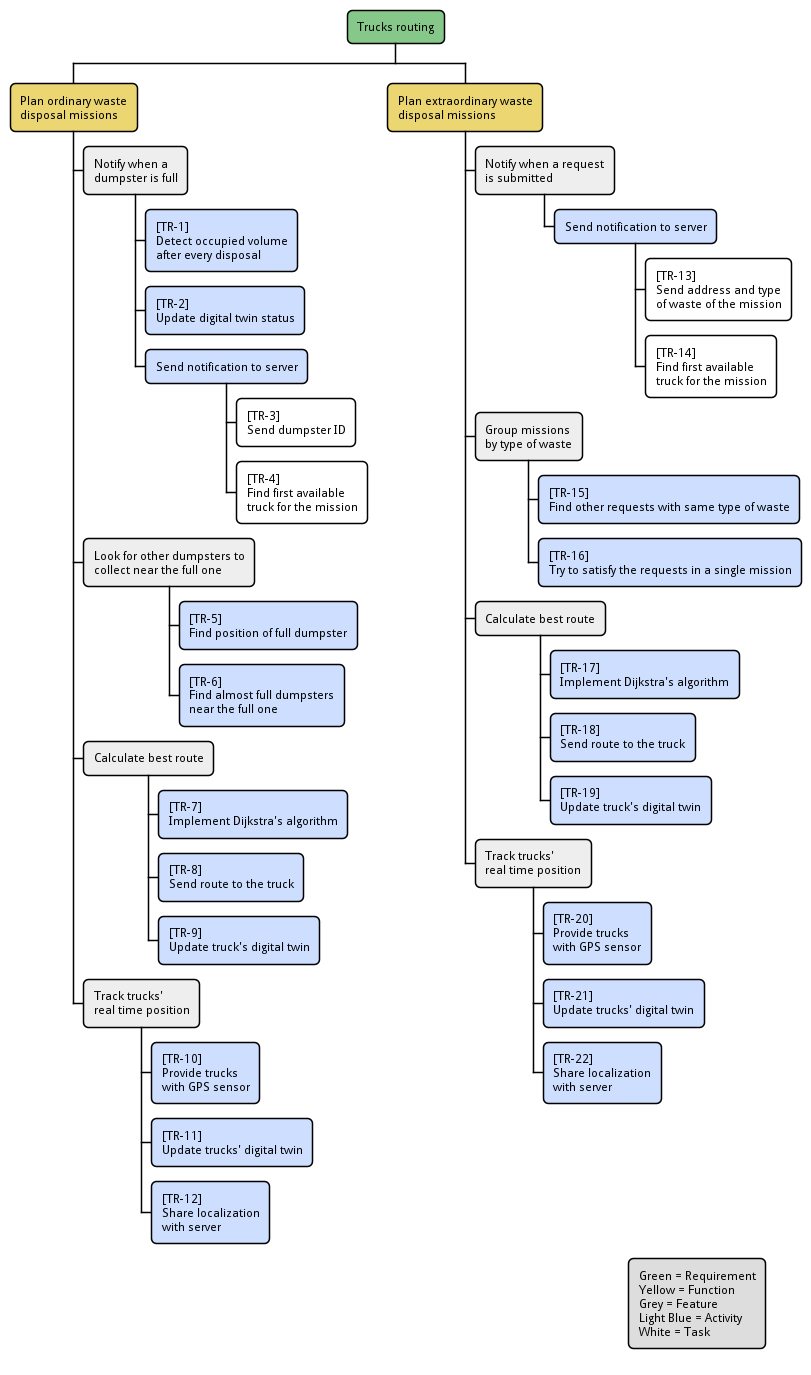
\includegraphics[width=\textwidth]{../img/wbs-trucks-routing.pm}
    \caption{\textit{Work Breakdown Structure} del \textbf{Trucks Routing}. \hyperlink{back:wbs-trucks-routing}{Torna indietro}.}
    \label{fig:wbs-trucks-routing}
\end{figure}

\begin{figure}[H]
    \centering
    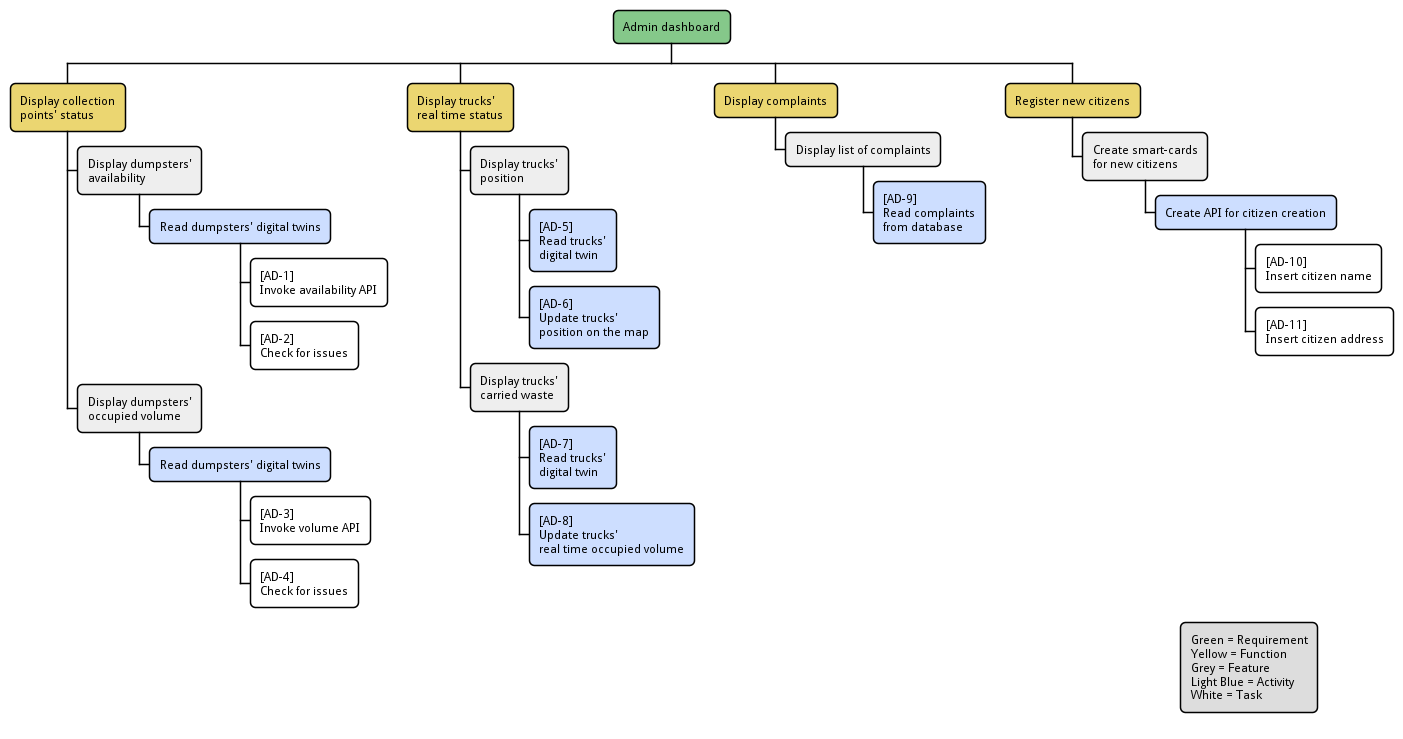
\includegraphics[width=\textwidth]{../img/wbs-admin-dashboard.pm}
    \caption{\textit{Work Breakdown Structure} della \textbf{Admin Dashboard}. \hyperlink{back:wbs-admin-dashboard}{Torna indietro}.}
    \label{fig:wbs-admin-dashboard}
\end{figure}

\begin{figure}[H]
    \centering
    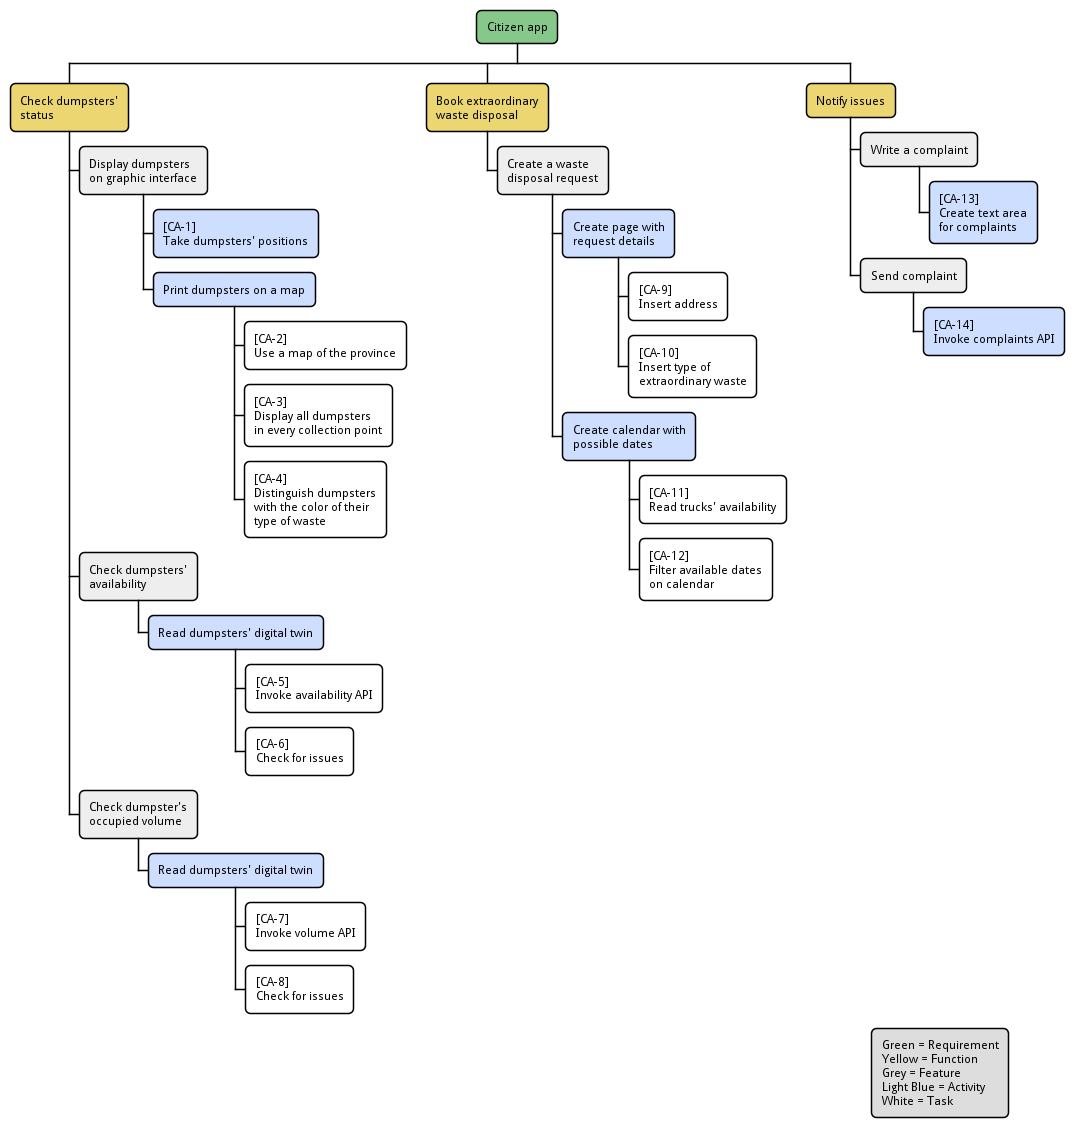
\includegraphics[width=\textwidth]{../img/wbs-citizen-app.pm}
    \caption{\textit{Work Breakdown Structure} della \textbf{Citizen App}. \hyperlink{back:wbs-citizen-app}{Torna indietro}.}
    \label{fig:wbs-citizen-app}
\end{figure}

\begin{figure}[H]
    \centering
    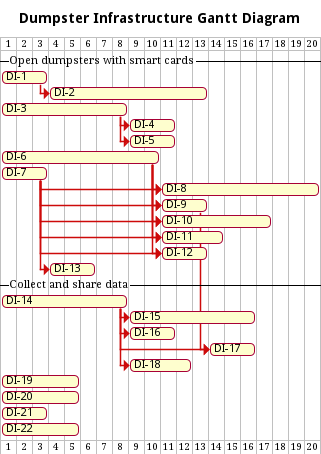
\includegraphics[width=\textwidth]{../img/gantt-dumpster-infrastructure.pm}
    \caption{Project Network Diagram contenente le attività e i task per portare a termine la \textit{Dumpster Infrastructure}. \hyperlink{back:gantt-dumpster-infrastructure}{Torna indietro}.}
    \label{fig:gantt-dumpster-infrastructure}
\end{figure}

\begin{figure}[H]
    \centering
    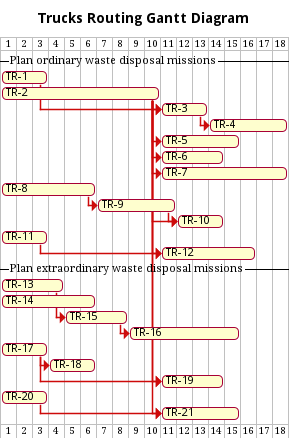
\includegraphics[width=\textwidth]{../img/gantt-trucks-routing.pm}
    \caption{Project Network Diagram contenente le attività e i task per portare a termine il \textit{Trucks Routing}. \hyperlink{back:gantt-trucks-routing}{Torna indietro}.}
    \label{fig:gantt-trucks-routing}
\end{figure}

\begin{figure}[H]
    \centering
    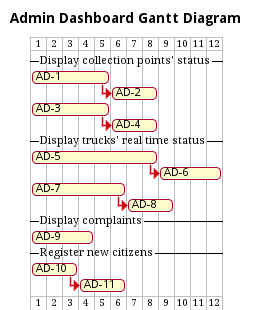
\includegraphics[width=\textwidth]{../img/gantt-admin-dashboard.pm}
    \caption{Project Network Diagram contenente le attività e i task per portare a termine la \textit{Admin Dashboard}. \hyperlink{back:gantt-admin-dashboard}{Torna indietro}.}
    \label{fig:gantt-admin-dashboard}
\end{figure}

\begin{figure}[H]
    \centering
    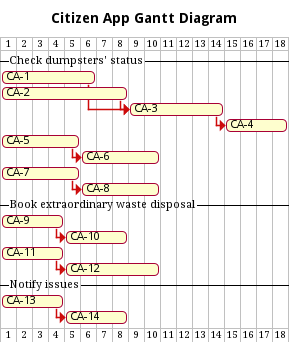
\includegraphics[width=\textwidth]{../img/gantt-citizen-app.pm}
    \caption{Project Network Diagram contenente le attività e i task per portare a termine la \textit{Citizen App}. \hyperlink{back:gantt-citizen-app}{Torna indietro}.}
    \label{fig:gantt-citizen-app}
\end{figure}

\begin{figure}[H]
    \centering
    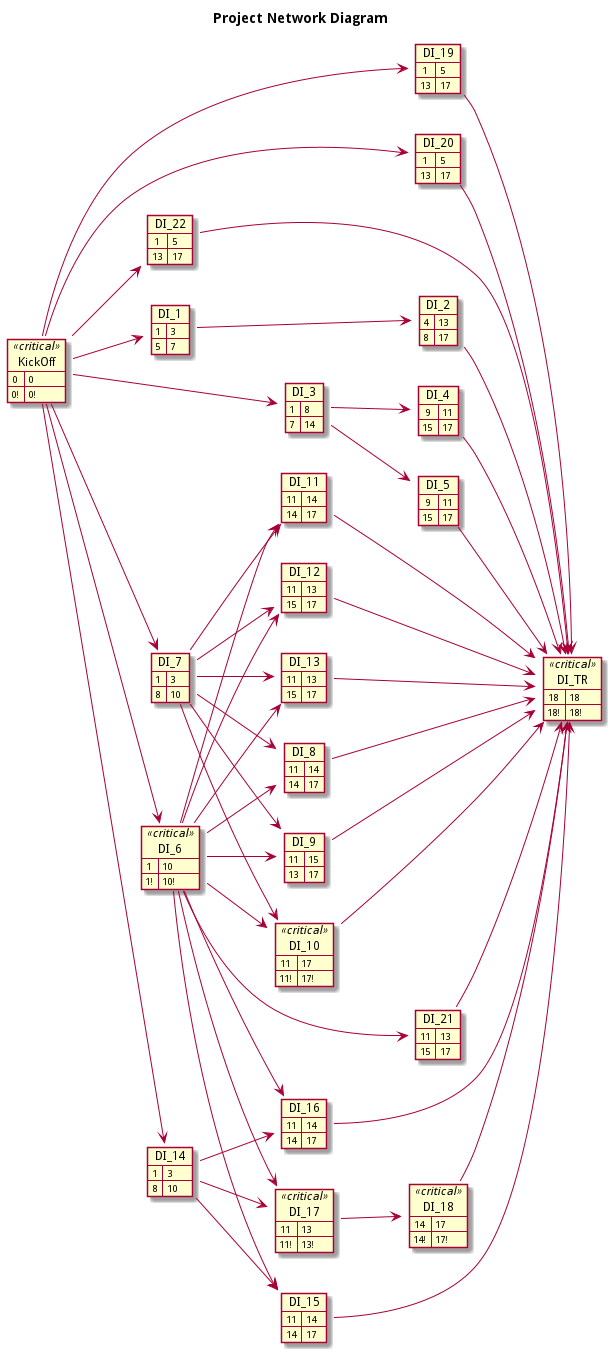
\includegraphics[width=\textwidth]{../img/pert-diagram.pm}
    \caption{Diagramma di PERT per l'individuazione del \textit{critical path}. \hyperlink{back:pert-diagram}{Torna indietro}.}
    \label{fig:pert-diagram}
\end{figure}

\begin{figure}[H]
    \centering
    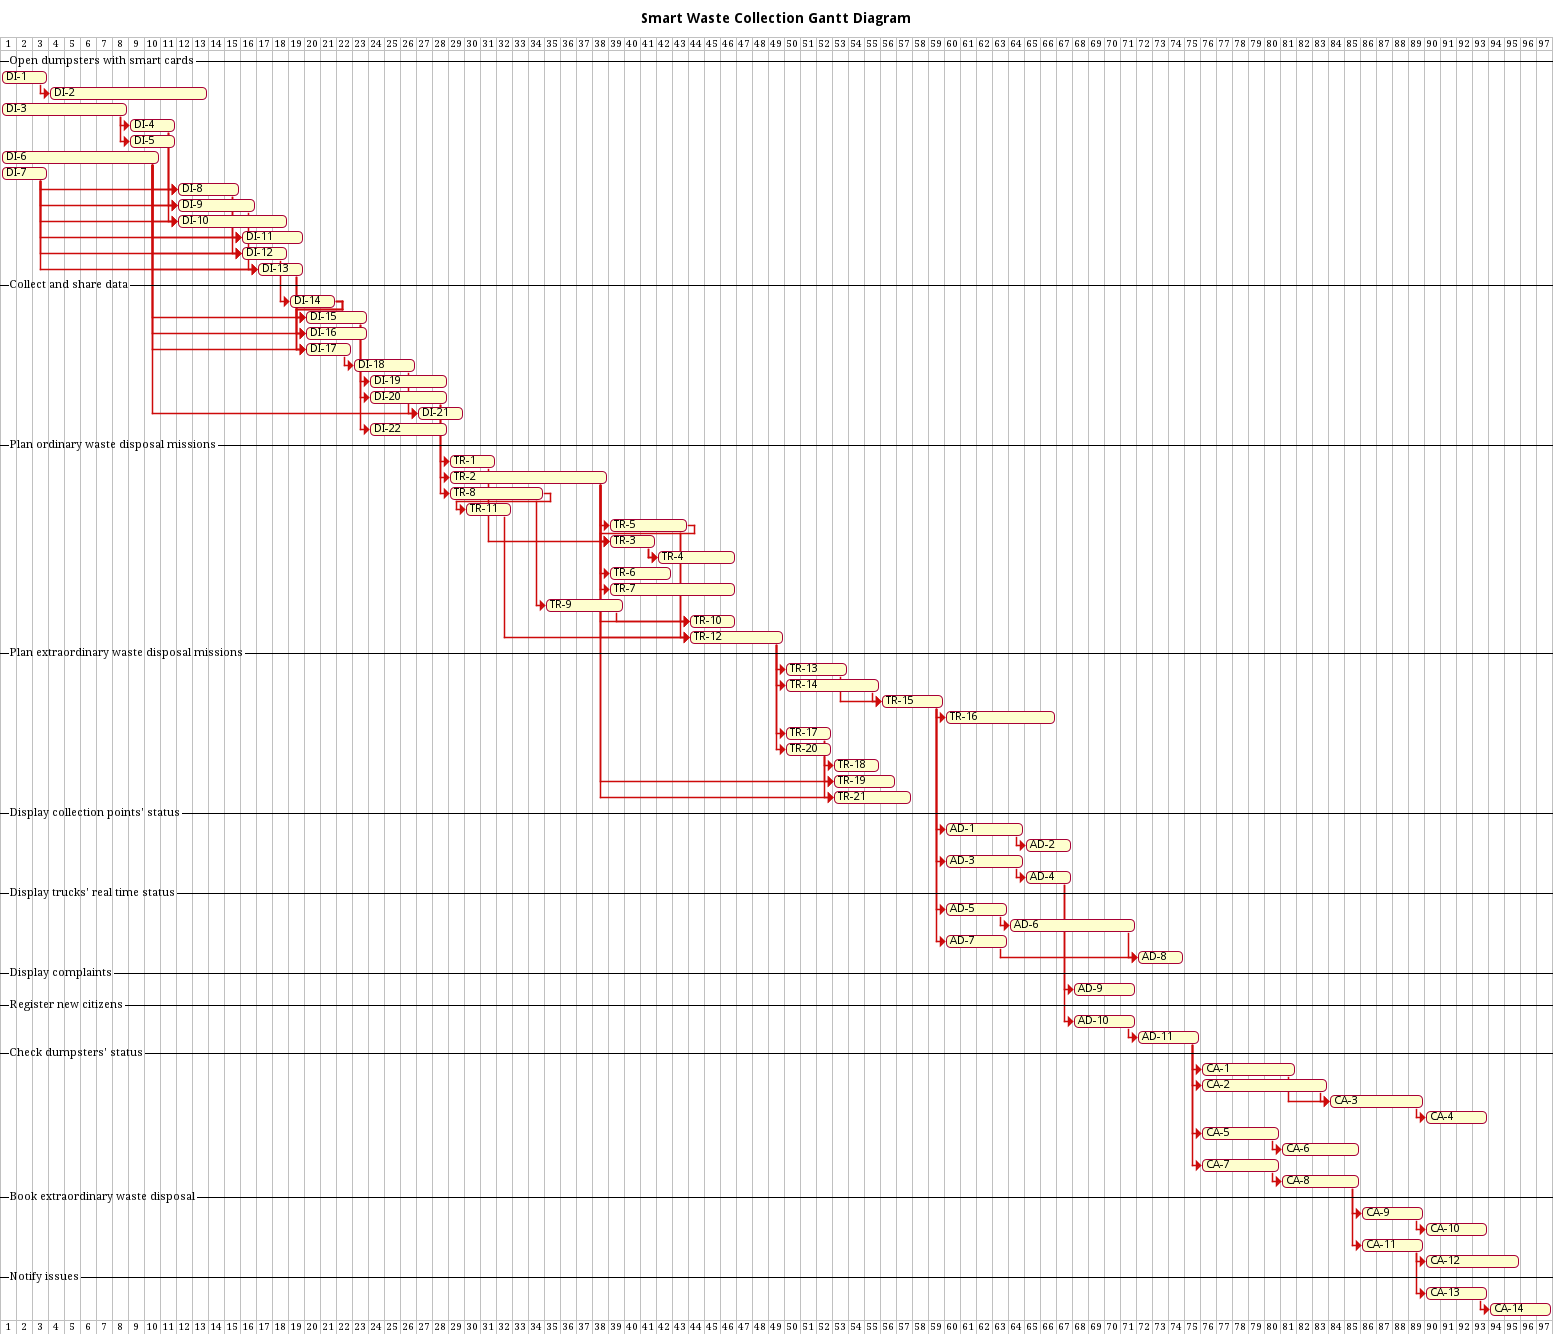
\includegraphics[width=\textwidth]{../img/gantt.pm}
    \caption{Diagramma Gantt di tutti i task del progetto svolgendo al massimo 4 attività in parallelo.  \hyperlink{back:gantt}{Torna indietro}.}
    \label{fig:gantt}
\end{figure}

\begin{figure}[H]
    \centering
    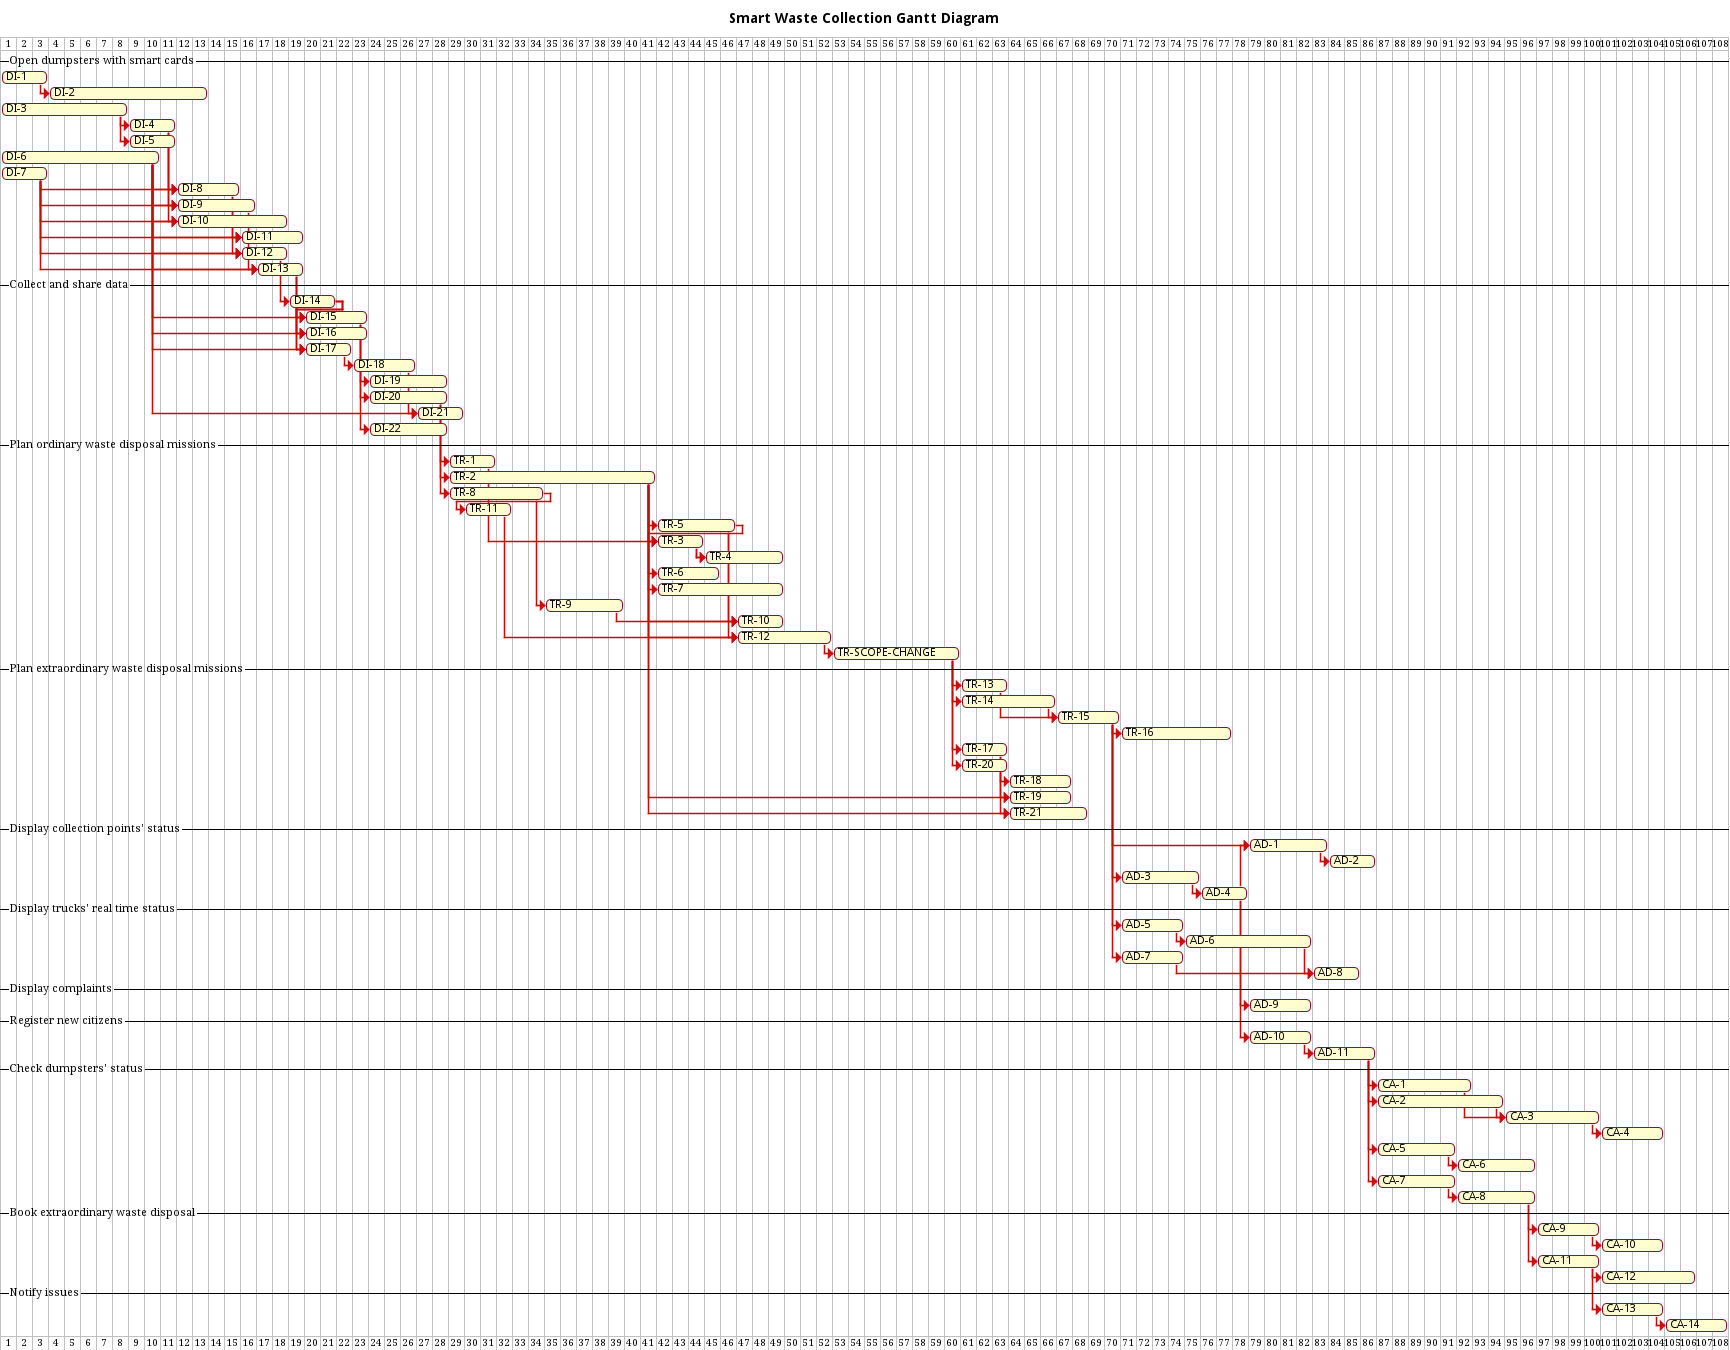
\includegraphics[width=\textwidth]{../img/gantt-redefinition.pm}
    \caption{Diagramma Gantt di tutti i task del progetto in seguito all'applicazione del cambiamento richiesto dal cliente.  \hyperlink{back:gantt-redefinition}{Torna indietro}.}
    \label{fig:gantt-redefinition}
\end{figure}
